\documentclass[10pt  ,usenames, dvipsnames]{article}\usepackage[]{graphicx}\usepackage[]{color}
%% maxwidth is the original width if it is less than linewidth
%% otherwise use linewidth (to make sure the graphics do not exceed the margin)
\makeatletter
\def\maxwidth{ %
  \ifdim\Gin@nat@width>\linewidth
    \linewidth
  \else
    \Gin@nat@width
  \fi
}
\makeatother

\definecolor{fgcolor}{rgb}{0.345, 0.345, 0.345}
\newcommand{\hlnum}[1]{\textcolor[rgb]{0.686,0.059,0.569}{#1}}%
\newcommand{\hlstr}[1]{\textcolor[rgb]{0.192,0.494,0.8}{#1}}%
\newcommand{\hlcom}[1]{\textcolor[rgb]{0.678,0.584,0.686}{\textit{#1}}}%
\newcommand{\hlopt}[1]{\textcolor[rgb]{0,0,0}{#1}}%
\newcommand{\hlstd}[1]{\textcolor[rgb]{0.345,0.345,0.345}{#1}}%
\newcommand{\hlkwa}[1]{\textcolor[rgb]{0.161,0.373,0.58}{\textbf{#1}}}%
\newcommand{\hlkwb}[1]{\textcolor[rgb]{0.69,0.353,0.396}{#1}}%
\newcommand{\hlkwc}[1]{\textcolor[rgb]{0.333,0.667,0.333}{#1}}%
\newcommand{\hlkwd}[1]{\textcolor[rgb]{0.737,0.353,0.396}{\textbf{#1}}}%
\let\hlipl\hlkwb

\usepackage{framed}
\makeatletter
\newenvironment{kframe}{%
 \def\at@end@of@kframe{}%
 \ifinner\ifhmode%
  \def\at@end@of@kframe{\end{minipage}}%
  \begin{minipage}{\columnwidth}%
 \fi\fi%
 \def\FrameCommand##1{\hskip\@totalleftmargin \hskip-\fboxsep
 \colorbox{shadecolor}{##1}\hskip-\fboxsep
     % There is no \\@totalrightmargin, so:
     \hskip-\linewidth \hskip-\@totalleftmargin \hskip\columnwidth}%
 \MakeFramed {\advance\hsize-\width
   \@totalleftmargin\z@ \linewidth\hsize
   \@setminipage}}%
 {\par\unskip\endMakeFramed%
 \at@end@of@kframe}
\makeatother

\definecolor{shadecolor}{rgb}{.97, .97, .97}
\definecolor{messagecolor}{rgb}{0, 0, 0}
\definecolor{warningcolor}{rgb}{1, 0, 1}
\definecolor{errorcolor}{rgb}{1, 0, 0}
\newenvironment{knitrout}{}{} % an empty environment to be redefined in TeX

\usepackage{alltt}
\usepackage{graphicx, verbatim}
\usepackage{amsmath}
\usepackage{amssymb}
\usepackage{amscd}
\usepackage{lipsum}
\usepackage{todonotes}
\usepackage[tableposition=top]{caption}
\usepackage{ifthen}
\usepackage[utf8]{inputenc}
\usepackage{graphicx}
\usepackage{caption}
\usepackage{listings}
\usepackage{color}
\setlength{\textwidth}{6.5in} 
\setlength{\textheight}{9in}
\setlength{\oddsidemargin}{0in} 
\setlength{\evensidemargin}{0in}
\setlength{\topmargin}{-1.5cm}
\setlength{\parindent}{0cm}
\usepackage{setspace}
\usepackage{float}
\usepackage{amssymb}
\usepackage[utf8]{inputenc}
\usepackage{fancyhdr}
\usepackage{tabularx}
\usepackage{lmodern} % for bold teletype font
\usepackage{minted}
\usepackage{underscore}
\usepackage{pdfpages}
\usepackage{graphicx}

\usepackage{hyperref}
\hypersetup{
  colorlinks   = true, %Colours links instead of ugly boxes
  urlcolor     = blue, %Colour for external hyperlinks
  linkcolor    = blue, %Colour of internal links
  citecolor   = red %Colour of citations
}

%\fancyhf{}
\rfoot{Andrew Tait \thepage}
\singlespacing
\usepackage[affil-it]{authblk} 
\usepackage{etoolbox}
\usepackage{lmodern}


% Notice the following package, it will help you cite papers
\usepackage[backend=bibtex ,sorting=none]{biblatex}
\bibliography{references}

\begin{filecontents*}{references.bib}

\end{filecontents*}
\IfFileExists{upquote.sty}{\usepackage{upquote}}{}
\begin{document}


\title{\LARGE Coursework  \\ Advanced Data Science (CMM536)}

\author{Andrew Tait, \textit{\href{1504693@rgu.ac.uk}{1504693@rgu.ac.uk}}}
\maketitle
% \begin{flushleft} \today \end{flushleft} 
\noindent\rule{16cm}{0.4pt}
%\underline{\hspace{3cm}
\ \\
%\thispagestyle{empty}

\section{Research}
The paper that was chosen for this work is \cite{PHRIDVIRAJ2014255}. The authors provided a full review on different streaming algorithms and method that handle data mining. Below is a review of this paper that includes problem statement, related work and methods applied.

\subsection{Problem Statement}
The process of data mining is to discover otherwise hidden information and patterns from already existing data. What makes this complicated when it comes to data streams is that unlike a traditional relation database or data warehouse there isn't a pre-defined structure. This paper outlines an algorithm that could possibly overcomes these difficulties.

\subsection{Relevant Work}
There is numerous related works and research in the field of data streaming. For instance the ACM KDDD international conference held in 2010, outlined the problem of finding the top-k frequent items in a data stream with flexible sliding widows. This would be only to mine the top-k frequent items, not reporting on all frequent items.

\subsection{Methods}
The paper outlines the issues that the new data streaming algorithm may face. This included memory constraint, data prepossessing choice of data structure, identifying data distributions and target concepts and dimensional reduction.
These are import issues to cover as they will reduce the efficiency and overall accuracy of the data streaming algorithm.

\subsection{Results}
The algorithm produces a decision tree which it outlines the nodes that are active/live as black, killed nodes as red and green nodes on the first level to indicate that they are not closed. It produces an more effective decision tree it only looks for the top-k frequent items in the decision and discards the rest.

\subsection{Conclusion}
As the subject matter is dealing with an unlimited amount of information, whether this will be from social media streams or general information retrieval. There is still problem to overcome with clustering, classification and topic detection in terms of data streaming. The proposed algorithm provides a starting point by creating a decision tree of the top-k frequent items.


\clearpage



\section {Data Streams}

\subsection{Dataset Choice}

The dataset that has been chosen for this part of the coursework is the 'adult' dataset. This is available on the UCI repository. It has been proved to a good evaluation of classification methods

\url{https://archive.ics.uci.edu/ml/datasets/adult}



\subsection{Data Exploration}

The main purpose of the adult dataset is to find out which characteristics of the us population affect if their income is either <=$50k or >=$50k



To start off I will clear the RStudio environment and import the required libraries.

\begin{knitrout}
\definecolor{shadecolor}{rgb}{0.969, 0.969, 0.969}\color{fgcolor}\begin{kframe}
\begin{alltt}
\hlcom{#Clean RStudio Environment}
\hlkwd{rm}\hlstd{(}\hlkwc{list} \hlstd{=} \hlkwd{ls}\hlstd{())}

\hlcom{#Import librarys}
\hlkwd{library}\hlstd{(caret)}
\hlkwd{library}\hlstd{(partykit)}
\hlkwd{library}\hlstd{(mlbench)}
\hlkwd{library}\hlstd{(RWeka)}
\hlkwd{library}\hlstd{(C50)}
\hlkwd{library}\hlstd{(datasets)}
\hlkwd{library}\hlstd{(rpart)}
\hlkwd{library}\hlstd{(ggplot2)}
\hlkwd{library}\hlstd{(data.table)}
\hlkwd{library}\hlstd{(stream)}
\hlkwd{library}\hlstd{(mlbench)}
\hlkwd{library}\hlstd{(doParallel)}
\hlkwd{library}\hlstd{(streamMOA)}
\hlkwd{library}\hlstd{(e1071)}
\hlkwd{library}\hlstd{(RMOA)}
\hlkwd{library}\hlstd{(ROCR)}
\hlkwd{library}\hlstd{(tm)}
\hlkwd{library}\hlstd{(wordcloud)}
\hlkwd{library}\hlstd{(wordcloud,}\hlkwc{quietly}\hlstd{=}\hlnum{TRUE}\hlstd{)}
\hlkwd{library}\hlstd{(RColorBrewer,}\hlkwc{quietly}\hlstd{=}\hlnum{TRUE}\hlstd{)}
\end{alltt}
\end{kframe}
\end{knitrout}



Then set the working directory to the coursework folder

\begin{knitrout}
\definecolor{shadecolor}{rgb}{0.969, 0.969, 0.969}\color{fgcolor}\begin{kframe}
\begin{alltt}
\hlcom{#Set working directory}
\hlkwd{setwd}\hlstd{(}\hlstr{"~/CMM536 Advanced Data Science/Coursework/CMM536_Coursework"}\hlstd{)}
\end{alltt}
\end{kframe}
\end{knitrout}



\clearpage

In order to the import the adult dataset, the feature names first need to be defined.
\begin{knitrout}
\definecolor{shadecolor}{rgb}{0.969, 0.969, 0.969}\color{fgcolor}\begin{kframe}
\begin{alltt}
\hlcom{#Feature names}
\hlstd{adultNames} \hlkwb{<-} \hlkwd{c}\hlstd{(}\hlstr{"age"}\hlstd{,} \hlstr{"workclass"}\hlstd{,} \hlstr{"fblwgt"}\hlstd{,}
                \hlstr{"education"}\hlstd{,} \hlstr{"education-num"}\hlstd{,}
                \hlstr{"martial-status"}\hlstd{,}
                \hlstr{"occupation"}\hlstd{,}
                \hlstr{"relationship"}\hlstd{,}
                \hlstr{"race"}\hlstd{,}
                \hlstr{"sex"}\hlstd{,}
                \hlstr{"captial-gain"}\hlstd{,}
                \hlstr{"captain-loss"}\hlstd{,}
                \hlstr{"hours-per-week"}\hlstd{,}
                \hlstr{"native-country"}\hlstd{,}
                \hlstr{"class"}\hlstd{)}
\end{alltt}
\end{kframe}
\end{knitrout}



The adult dataset is then imported from adult.data file:
\begin{knitrout}
\definecolor{shadecolor}{rgb}{0.969, 0.969, 0.969}\color{fgcolor}\begin{kframe}
\begin{alltt}
\hlcom{#Import datasets}
\hlstd{adult} \hlkwb{<-} \hlkwd{read.table}\hlstd{(}\hlstr{"data/adult.data"} \hlstd{,}\hlkwc{header} \hlstd{=} \hlnum{FALSE}\hlstd{,} \hlkwc{sep} \hlstd{=} \hlstr{","}\hlstd{,}
                         \hlkwc{strip.white} \hlstd{=} \hlnum{TRUE}\hlstd{,} \hlkwc{col.names} \hlstd{= adultNames,}
                         \hlkwc{na.strings} \hlstd{=} \hlstr{"?"}\hlstd{,} \hlkwc{stringsAsFactors} \hlstd{=} \hlnum{TRUE}\hlstd{)}
\end{alltt}
\end{kframe}
\end{knitrout}




Now the adult dataset is imported, it's time for some basic exploration

Number of rows (instances) in the dataset

\begin{knitrout}
\definecolor{shadecolor}{rgb}{0.969, 0.969, 0.969}\color{fgcolor}\begin{kframe}
\begin{alltt}
\hlkwd{nrow}\hlstd{(adult)}
\end{alltt}
\end{kframe}
\end{knitrout}

\begin{knitrout}
\definecolor{shadecolor}{rgb}{0.969, 0.969, 0.969}\color{fgcolor}\begin{kframe}
\begin{verbatim}
## [1] 32561
\end{verbatim}
\end{kframe}
\end{knitrout}

The number of columns (features)

\begin{knitrout}
\definecolor{shadecolor}{rgb}{0.969, 0.969, 0.969}\color{fgcolor}\begin{kframe}
\begin{alltt}
\hlkwd{ncol}\hlstd{(adult)}
\end{alltt}
\end{kframe}
\end{knitrout}

\begin{knitrout}
\definecolor{shadecolor}{rgb}{0.969, 0.969, 0.969}\color{fgcolor}\begin{kframe}
\begin{verbatim}
## [1] 15
\end{verbatim}
\end{kframe}
\end{knitrout}

Summary of the adult dataset:

\begin{knitrout}
\definecolor{shadecolor}{rgb}{0.969, 0.969, 0.969}\color{fgcolor}\begin{kframe}
\begin{alltt}
\hlcom{#inspect dataset}
\hlkwd{str}\hlstd{(adult)}
\end{alltt}
\end{kframe}
\end{knitrout}

\begin{knitrout}
\definecolor{shadecolor}{rgb}{0.969, 0.969, 0.969}\color{fgcolor}\begin{kframe}
\begin{verbatim}
## 'data.frame':	32561 obs. of  15 variables:
##  $ age           : int  39 50 38 53 28 37 49 52 31 42 ...
##  $ workclass     : Factor w/ 8 levels "Federal-gov",..: 7 6 4 4 4 4 4 6 4 4 ...
##  $ fblwgt        : int  77516 83311 215646 234721 338409 284582 160187 209642 45781 159449 ...
##  $ education     : Factor w/ 16 levels "10th","11th",..: 10 10 12 2 10 13 7 12 13 10 ...
##  $ education.num : int  13 13 9 7 13 14 5 9 14 13 ...
##  $ martial.status: Factor w/ 7 levels "Divorced","Married-AF-spouse",..: 5 3 1 3 3 3 4 3 5 3 ...
##  $ occupation    : Factor w/ 14 levels "Adm-clerical",..: 1 4 6 6 10 4 8 4 10 4 ...
##  $ relationship  : Factor w/ 6 levels "Husband","Not-in-family",..: 2 1 2 1 6 6 2 1 2 1 ...
##  $ race          : Factor w/ 5 levels "Amer-Indian-Eskimo",..: 5 5 5 3 3 5 3 5 5 5 ...
##  $ sex           : Factor w/ 2 levels "Female","Male": 2 2 2 2 1 1 1 2 1 2 ...
##  $ captial.gain  : int  2174 0 0 0 0 0 0 0 14084 5178 ...
##  $ captain.loss  : int  0 0 0 0 0 0 0 0 0 0 ...
##  $ hours.per.week: int  40 13 40 40 40 40 16 45 50 40 ...
##  $ native.country: Factor w/ 41 levels "Cambodia","Canada",..: 39 39 39 39 5 39 23 39 39 39 ...
##  $ class         : Factor w/ 2 levels "<=50K",">50K": 1 1 1 1 1 1 1 2 2 2 ...
\end{verbatim}
\end{kframe}
\end{knitrout}



Now that some basic data exploration is covered, next to inspect the dataset a bit further. Starting with the class distribution in the adult dataset, see (Figure~\ref{fig1})

\begin{knitrout}
\definecolor{shadecolor}{rgb}{0.969, 0.969, 0.969}\color{fgcolor}\begin{kframe}
\begin{alltt}
\hlcom{#Class Distribution}
\hlkwd{barplot}\hlstd{(}\hlkwd{table}\hlstd{(adult}\hlopt{$}\hlstd{class))}
\end{alltt}
\end{kframe}
\end{knitrout}

\begin{figure}[H]
\begin{center}
\begin{knitrout}
\definecolor{shadecolor}{rgb}{0.969, 0.969, 0.969}\color{fgcolor}
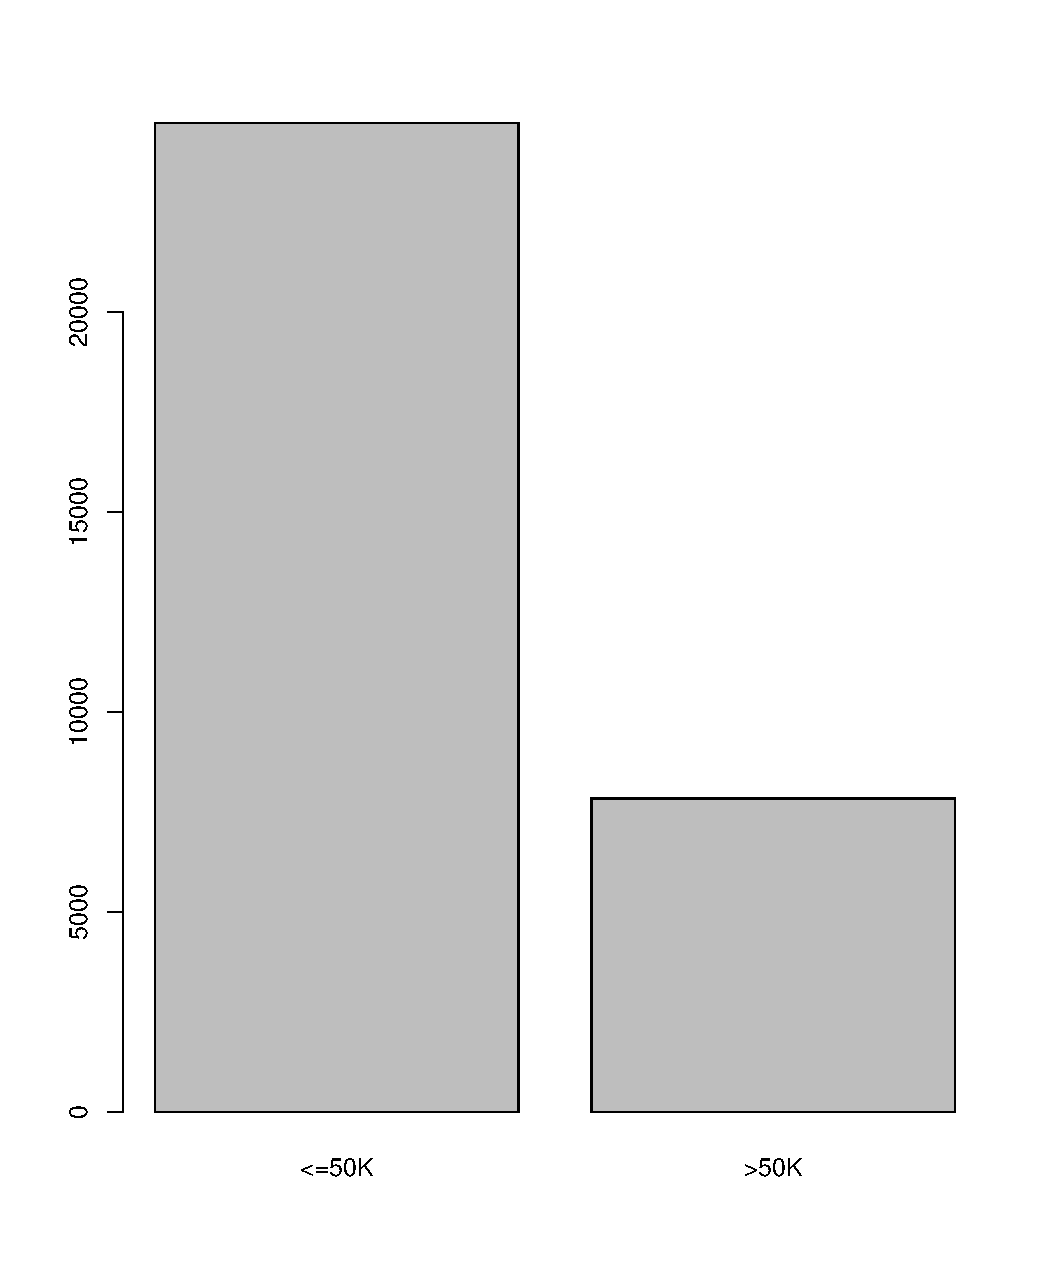
\includegraphics[width=.76\linewidth]{figure/unnamed-chunk-16-1} 

\end{knitrout}
\caption {Barplot of Class Distribution}
\label{fig1}
\end {center}
\end {figure}

As the barplot clearly shows, the adult dataset is highly unbalanced with <=50k being the majority class by a large margin!

\clearpage

\subsection{Build Classifier}

\subsubsection{Pre-Processing}
Before the adult dataset can classified, some pre-processing is required first.

The dataset is checked for missing values ('?')
\begin{knitrout}
\definecolor{shadecolor}{rgb}{0.969, 0.969, 0.969}\color{fgcolor}\begin{kframe}
\begin{alltt}
\hlcom{#Check for missing values ('?')}
\hlkwd{table}\hlstd{(}\hlkwd{complete.cases} \hlstd{(adult))}
\end{alltt}
\end{kframe}
\end{knitrout}

\begin{knitrout}
\definecolor{shadecolor}{rgb}{0.969, 0.969, 0.969}\color{fgcolor}\begin{kframe}
\begin{verbatim}
## 
## FALSE  TRUE 
##  2399 30162
\end{verbatim}
\end{kframe}
\end{knitrout}

As shown above there are missing values in the workclass,occupation and class columns. so these are removed.

\begin{knitrout}
\definecolor{shadecolor}{rgb}{0.969, 0.969, 0.969}\color{fgcolor}\begin{kframe}
\begin{alltt}
\hlstd{cleanadult} \hlkwb{=} \hlstd{adult[}\hlopt{!}\hlkwd{is.na}\hlstd{(adult}\hlopt{$}\hlstd{workclass)}\hlopt{& !}\hlkwd{is.na}\hlstd{(adult}\hlopt{$}\hlstd{occupation)} \hlopt{& !}\hlkwd{is.na}\hlstd{(adult}\hlopt{$}\hlstd{class),]}
\end{alltt}
\end{kframe}
\end{knitrout}




The flwgt feature is also removed as it's not required.

\begin{knitrout}
\definecolor{shadecolor}{rgb}{0.969, 0.969, 0.969}\color{fgcolor}\begin{kframe}
\begin{alltt}
\hlcom{#Remove flwgt feature}
\hlstd{cleanadult}\hlopt{$}\hlstd{fblwgt} \hlkwb{=} \hlkwa{NULL}
\end{alltt}
\end{kframe}
\end{knitrout}



Lets inspect the cleanadult dataframe before going further:

\begin{knitrout}
\definecolor{shadecolor}{rgb}{0.969, 0.969, 0.969}\color{fgcolor}\begin{kframe}
\begin{alltt}
\hlkwd{str}\hlstd{(cleanadult)}
\end{alltt}
\end{kframe}
\end{knitrout}

\begin{knitrout}
\definecolor{shadecolor}{rgb}{0.969, 0.969, 0.969}\color{fgcolor}\begin{kframe}
\begin{verbatim}
## 'data.frame':	30718 obs. of  14 variables:
##  $ age           : int  39 50 38 53 28 37 49 52 31 42 ...
##  $ workclass     : Factor w/ 8 levels "Federal-gov",..: 7 6 4 4 4 4 4 6 4 4 ...
##  $ education     : Factor w/ 16 levels "10th","11th",..: 10 10 12 2 10 13 7 12 13 10 ...
##  $ education.num : int  13 13 9 7 13 14 5 9 14 13 ...
##  $ martial.status: Factor w/ 7 levels "Divorced","Married-AF-spouse",..: 5 3 1 3 3 3 4 3 5 3 ...
##  $ occupation    : Factor w/ 14 levels "Adm-clerical",..: 1 4 6 6 10 4 8 4 10 4 ...
##  $ relationship  : Factor w/ 6 levels "Husband","Not-in-family",..: 2 1 2 1 6 6 2 1 2 1 ...
##  $ race          : Factor w/ 5 levels "Amer-Indian-Eskimo",..: 5 5 5 3 3 5 3 5 5 5 ...
##  $ sex           : Factor w/ 2 levels "Female","Male": 2 2 2 2 1 1 1 2 1 2 ...
##  $ captial.gain  : int  2174 0 0 0 0 0 0 0 14084 5178 ...
##  $ captain.loss  : int  0 0 0 0 0 0 0 0 0 0 ...
##  $ hours.per.week: int  40 13 40 40 40 40 16 45 50 40 ...
##  $ native.country: Factor w/ 41 levels "Cambodia","Canada",..: 39 39 39 39 5 39 23 39 39 39 ...
##  $ class         : Factor w/ 2 levels "<=50K",">50K": 1 1 1 1 1 1 1 2 2 2 ...
\end{verbatim}
\end{kframe}
\end{knitrout}


\clearpage

As the adult dataset is a mixture of factors, integers and characters, I decided that transforming the dataset into binary. This will be create features based on every possible value in the dataset.

The cleanadult dataframe is first copied and the class is removed (it's not being transformed into binary)

\begin{knitrout}
\definecolor{shadecolor}{rgb}{0.969, 0.969, 0.969}\color{fgcolor}\begin{kframe}
\begin{alltt}
\hlcom{#Copy dataset}
\hlstd{noClass} \hlkwb{<-}\hlstd{cleanadult}
\hlcom{#Remove class as it is not being transformed to binary}
\hlstd{noClass}\hlopt{$}\hlstd{class} \hlkwb{<-} \hlkwa{NULL}
\end{alltt}
\end{kframe}
\end{knitrout}




Then the noClass dataframe is transformed into binary

\begin{knitrout}
\definecolor{shadecolor}{rgb}{0.969, 0.969, 0.969}\color{fgcolor}\begin{kframe}
\begin{alltt}
\hlstd{binaryVars} \hlkwb{<-} \hlstd{caret}\hlopt{::}\hlkwd{dummyVars}\hlstd{(}\hlopt{~} \hlstd{.,} \hlkwc{data} \hlstd{= noClass)}
\hlstd{newAdult} \hlkwb{<-} \hlkwd{predict}\hlstd{(binaryVars,} \hlkwc{newdata} \hlstd{= noClass)}
\end{alltt}
\end{kframe}
\end{knitrout}



The class feature is then added to the binarised dataset
\begin{knitrout}
\definecolor{shadecolor}{rgb}{0.969, 0.969, 0.969}\color{fgcolor}\begin{kframe}
\begin{alltt}
\hlcom{#add class to binarised dataset}
\hlstd{binAdult} \hlkwb{<-}\hlkwd{cbind}\hlstd{(newAdult, cleanadult[}\hlnum{14}\hlstd{])}
\end{alltt}
\end{kframe}
\end{knitrout}



Any rows with NA values after being binary transformed.
\begin{knitrout}
\definecolor{shadecolor}{rgb}{0.969, 0.969, 0.969}\color{fgcolor}\begin{kframe}
\begin{alltt}
\hlcom{#remove any rows with NA values}
\hlstd{row.has.na} \hlkwb{<-} \hlkwd{apply}\hlstd{(binAdult,} \hlnum{1}\hlstd{,} \hlkwa{function}\hlstd{(}\hlkwc{x}\hlstd{)\{}\hlkwd{any}\hlstd{(}\hlkwd{is.na}\hlstd{(x))\})}
\hlkwd{sum}\hlstd{(row.has.na)}
\hlstd{binAdult} \hlkwb{<-} \hlstd{binAdult[}\hlopt{!}\hlstd{row.has.na,]}
\end{alltt}
\end{kframe}
\end{knitrout}

Number of NA rows removed.
\begin{knitrout}
\definecolor{shadecolor}{rgb}{0.969, 0.969, 0.969}\color{fgcolor}\begin{kframe}
\begin{verbatim}
## [1] 556
\end{verbatim}
\end{kframe}
\end{knitrout}

\clearpage

\subsubsection{Classification}

When it came to dividing the mushroom dataset into training and testing subsets, I decided to go with 80
percent training and 20 percent testing split as a starting point/baseline. 
Since the class distribution is unbalanced, I thought this split would cover the majority of cases.

\begin{knitrout}
\definecolor{shadecolor}{rgb}{0.969, 0.969, 0.969}\color{fgcolor}\begin{kframe}
\begin{alltt}
\hlcom{#split 80% training and 20% testing datasets}
\hlstd{inTrain} \hlkwb{<-} \hlkwd{createDataPartition}\hlstd{(}\hlkwc{y}\hlstd{=binAdult}\hlopt{$}\hlstd{class,} \hlkwc{p}\hlstd{=}\hlnum{0.8}\hlstd{,} \hlkwc{list}\hlstd{=}\hlnum{FALSE}\hlstd{)}

\hlcom{#Assign indexes to split the binAdult dataset into training and testing}
\hlstd{training} \hlkwb{<-} \hlstd{binAdult[inTrain,]}
\hlstd{testing} \hlkwb{<-} \hlstd{binAdult[inTrain,]}
\end{alltt}
\end{kframe}
\end{knitrout}




For the initial classifier I decided to go with the kNN Classifier as it has proven to be a good baseline in previous labs and exercises in R.
Before the classification begins, parallel processing is enabled to speed up this process.

\begin{knitrout}
\definecolor{shadecolor}{rgb}{0.969, 0.969, 0.969}\color{fgcolor}\begin{kframe}
\begin{alltt}
\hlcom{#Setup Parallel processing to speed up classification modelling}
\hlstd{cl} \hlkwb{<-} \hlkwd{makeCluster}\hlstd{(}\hlkwd{detectCores}\hlstd{(),} \hlkwc{type}\hlstd{=}\hlstr{'PSOCK'}\hlstd{)}
\hlkwd{registerDoParallel}\hlstd{(cl)}
\end{alltt}
\end{kframe}
\end{knitrout}



The train control is set to repeated-cross-validation with 10 folds and 3 repeats
\begin{knitrout}
\definecolor{shadecolor}{rgb}{0.969, 0.969, 0.969}\color{fgcolor}\begin{kframe}
\begin{alltt}
\hlstd{ctrl} \hlkwb{<-} \hlkwd{trainControl}\hlstd{(}\hlkwc{method} \hlstd{=} \hlstr{"repeatedcv"}\hlstd{,}
                     \hlkwc{repeats} \hlstd{=} \hlnum{3}\hlstd{,}
                     \hlkwc{number} \hlstd{=} \hlnum{10}\hlstd{,}
                     \hlkwc{verboseIter}\hlstd{=}\hlnum{TRUE}\hlstd{)}
\end{alltt}
\end{kframe}
\end{knitrout}



Next the seed is set to 1, in order to make the model reproducible and the kNN model is set up with the train control from above and k value set to 3.

\begin{knitrout}
\definecolor{shadecolor}{rgb}{0.969, 0.969, 0.969}\color{fgcolor}\begin{kframe}
\begin{alltt}
\hlcom{# ensure reproducibility of results by setting the seed to a known value}
\hlkwd{set.seed}\hlstd{(}\hlnum{1}\hlstd{)}
\hlcom{#use knn}
\hlstd{mod21.knn}\hlkwb{<-} \hlkwd{train}\hlstd{(class}\hlopt{~}\hlstd{.,} \hlkwc{data}\hlstd{=training,}
                  \hlkwc{method}\hlstd{=}\hlstr{"knn"}\hlstd{,} \hlkwc{tuneGrid}\hlstd{=}\hlkwd{expand.grid}\hlstd{(}\hlkwc{.k}\hlstd{=}\hlnum{3}\hlstd{),}\hlkwc{trControl}\hlstd{=ctrl)}
\end{alltt}
\end{kframe}
\end{knitrout}

\begin{knitrout}
\definecolor{shadecolor}{rgb}{0.969, 0.969, 0.969}\color{fgcolor}\begin{kframe}
\begin{verbatim}
## Aggregating results
## Fitting final model on full training set
\end{verbatim}
\end{kframe}
\end{knitrout}


\clearpage

Once the knn Model is complete, it’s time to analyse the results, first with a print of the kNNModel as shown below.
\begin{knitrout}
\definecolor{shadecolor}{rgb}{0.969, 0.969, 0.969}\color{fgcolor}\begin{kframe}
\begin{alltt}
\hlkwd{print}\hlstd{(mod21.knn)}
\end{alltt}
\end{kframe}
\end{knitrout}

\begin{knitrout}
\definecolor{shadecolor}{rgb}{0.969, 0.969, 0.969}\color{fgcolor}\begin{kframe}
\begin{verbatim}
## k-Nearest Neighbors 
## 
## 24131 samples
##   104 predictor
##     2 classes: '<=50K', '>50K' 
## 
## No pre-processing
## Resampling: Cross-Validated (10 fold, repeated 3 times) 
## Summary of sample sizes: 21717, 21718, 21719, 21718, 21718, 21718, ... 
## Resampling results:
## 
##   Accuracy   Kappa    
##   0.8361309  0.5541515
## 
## Tuning parameter 'k' was held constant at a value of 3
\end{verbatim}
\end{kframe}
\end{knitrout}

On first inspection, the knnModel produces an accuracy of 83.61\% and kappa value of 0.55. Further evaluation can be found in the next section.

\clearpage

\subsubsection {Evaluation}

To evaluate the module, a confusion matrix is produced by predicting the against the testing (20 percent of the total dataset ) subset.

\begin{knitrout}
\definecolor{shadecolor}{rgb}{0.969, 0.969, 0.969}\color{fgcolor}\begin{kframe}
\begin{alltt}
\hlcom{#Evaluation}
\hlstd{predictkNN} \hlkwb{<-} \hlkwd{predict}\hlstd{(mod21.knn,testing)}
\hlkwd{confusionMatrix}\hlstd{(predictkNN, testing}\hlopt{$}\hlstd{class)}
\end{alltt}
\end{kframe}
\end{knitrout}


\begin{knitrout}
\definecolor{shadecolor}{rgb}{0.969, 0.969, 0.969}\color{fgcolor}\begin{kframe}
\begin{verbatim}
## Confusion Matrix and Statistics
## 
##           Reference
## Prediction <=50K  >50K
##      <=50K 17026  1477
##      >50K   1098  4530
##                                           
##                Accuracy : 0.8933          
##                  95% CI : (0.8893, 0.8972)
##     No Information Rate : 0.7511          
##     P-Value [Acc > NIR] : < 2.2e-16       
##                                           
##                   Kappa : 0.7085          
##  Mcnemar's Test P-Value : 9.399e-14       
##                                           
##             Sensitivity : 0.9394          
##             Specificity : 0.7541          
##          Pos Pred Value : 0.9202          
##          Neg Pred Value : 0.8049          
##              Prevalence : 0.7511          
##          Detection Rate : 0.7056          
##    Detection Prevalence : 0.7668          
##       Balanced Accuracy : 0.8468          
##                                           
##        'Positive' Class : <=50K           
## 
\end{verbatim}
\end{kframe}
\end{knitrout}

As the confusion matrix shows that the kNNmodel produced an accuracy of 89.33\% when predicted against the training subset.

It correctly classified 17026 rows as <=50k and 4530 rows as >=50k.
However 1098 rows were incorrectly classified as <=50k and 1477 rows were incorrectly classified as >50k.

Overall it's a good start and could be improved upon further, with more computing resources and time to hand.

\clearpage

\subsection{Build Stream Classifier}

For the data streaming classifier, I used the binary adult dataset as used in the kNN model.

First the binary adult dataset is copied to a dataframe.

\begin{knitrout}
\definecolor{shadecolor}{rgb}{0.969, 0.969, 0.969}\color{fgcolor}\begin{kframe}
\begin{alltt}
\hlcom{#Pre-processing}
\hlcom{#copy the binary adult dataset}
\hlstd{df} \hlkwb{<-} \hlstd{binAdult}
\end{alltt}
\end{kframe}
\end{knitrout}



Next the control settings for the classification model are configured.

\begin{knitrout}
\definecolor{shadecolor}{rgb}{0.969, 0.969, 0.969}\color{fgcolor}\begin{kframe}
\begin{alltt}
\hlstd{ctrl} \hlkwb{<-} \hlkwd{MOAoptions}\hlstd{(}\hlkwc{model} \hlstd{=} \hlstr{"OCBoost"}\hlstd{,} \hlkwc{randomSeed} \hlstd{=} \hlnum{123456789}\hlstd{,} \hlkwc{ensembleSize} \hlstd{=} \hlnum{25}\hlstd{,}
                   \hlkwc{smoothingParameter} \hlstd{=} \hlnum{0.5}\hlstd{)}
\hlstd{mymodel} \hlkwb{<-} \hlkwd{OCBoost}\hlstd{(}\hlkwc{control} \hlstd{= ctrl)}
\hlstd{mymodel}
\end{alltt}
\end{kframe}
\end{knitrout}


\begin{knitrout}
\definecolor{shadecolor}{rgb}{0.969, 0.969, 0.969}\color{fgcolor}\begin{kframe}
\begin{verbatim}
## OCBoost modelling options: 
## MOA model name: Online Coordinate boosting for two classes evolving data streams.
##   - baseLearner: trees.HoeffdingTree   (Classifier to train.)
##   - ensembleSize: 25   (The number of models to boost.)
##   - smoothingParameter: 0.5   (Smoothing parameter.)
##   - randomSeed: 123456789   (Seed for random behaviour of the classifier.)
\end{verbatim}
\end{kframe}
\end{knitrout}

After setting the classification model, it's time to create the data stream and set some variables to control the iteration over the stream (see for loop)

\begin{knitrout}
\definecolor{shadecolor}{rgb}{0.969, 0.969, 0.969}\color{fgcolor}\begin{kframe}
\begin{alltt}
\hlcom{#Create datastream from the dataframe.}
\hlstd{dfStream} \hlkwb{<-}\hlkwd{datastream_dataframe}\hlstd{(}\hlkwc{data}\hlstd{=}\hlkwd{as.data.table}\hlstd{(df))}
\hlcom{#Set variables for stream iteration}
\hlstd{chunk} \hlkwb{<-} \hlnum{100}
\hlstd{turns} \hlkwb{<-} \hlstd{(}\hlkwd{nrow}\hlstd{(dfStream}\hlopt{$}\hlstd{data)}\hlopt{/}\hlstd{chunk)}\hlopt{-}\hlnum{1}
\hlstd{turns} \hlkwb{<-} \hlkwd{floor}\hlstd{(turns)}
\hlstd{position} \hlkwb{<-} \hlstd{chunk}
\end{alltt}
\end{kframe}
\end{knitrout}



Next a sample of the dataset is created (first 100 rows)

\begin{knitrout}
\definecolor{shadecolor}{rgb}{0.969, 0.969, 0.969}\color{fgcolor}\begin{kframe}
\begin{alltt}
\hlcom{#first sample (train)}
\hlstd{sample} \hlkwb{<-} \hlstd{dfStream}\hlopt{$}\hlkwd{get_points}\hlstd{(dfStream,} \hlkwc{n} \hlstd{=chunk,}
                             \hlkwc{outofpoints} \hlstd{=} \hlkwd{c}\hlstd{(}\hlstr{"stop"}\hlstd{,} \hlstr{"warn"}\hlstd{,} \hlstr{"ignore"}\hlstd{))}
\end{alltt}
\end{kframe}
\end{knitrout}




For verification that the sample and original rows are the same, the first 10 classes of each are displayed. Note there are 105 features from the binary dataset, so displaying them all will take up a lot of pages, so only the class is shown for simplicity.

\begin{knitrout}
\definecolor{shadecolor}{rgb}{0.969, 0.969, 0.969}\color{fgcolor}\begin{kframe}
\begin{alltt}
\hlkwd{head}\hlstd{(sample}\hlopt{$}\hlstd{class,}\hlnum{10}\hlstd{)}
\hlkwd{head}\hlstd{(df}\hlopt{$}\hlstd{class,}\hlnum{10}\hlstd{)}
\end{alltt}
\end{kframe}
\end{knitrout}

The first 10 classes of the sample chunk
\begin{knitrout}
\definecolor{shadecolor}{rgb}{0.969, 0.969, 0.969}\color{fgcolor}\begin{kframe}
\begin{verbatim}
##  [1] <=50K <=50K <=50K <=50K <=50K <=50K <=50K >50K  >50K  >50K 
## Levels: <=50K >50K
\end{verbatim}
\end{kframe}
\end{knitrout}

The first 10 classes of the df dataframe.
\begin{knitrout}
\definecolor{shadecolor}{rgb}{0.969, 0.969, 0.969}\color{fgcolor}\begin{kframe}
\begin{verbatim}
##  [1] <=50K <=50K <=50K <=50K <=50K <=50K <=50K >50K  >50K  >50K 
## Levels: <=50K >50K
\end{verbatim}
\end{kframe}
\end{knitrout}

With all the streaming data now setup, the model can be trained using the 1st chunk of data and then iterated against the whole of the data stream.

\begin{knitrout}
\definecolor{shadecolor}{rgb}{0.969, 0.969, 0.969}\color{fgcolor}\begin{kframe}
\begin{alltt}
\hlcom{##Train the first chunk}

\hlstd{myboostedclasifier} \hlkwb{<-} \hlkwd{trainMOA}\hlstd{(}\hlkwc{model}\hlstd{=mymodel,}
                      \hlkwc{formula} \hlstd{= class}\hlopt{~}\hlstd{.,}
                      \hlkwc{data} \hlstd{=} \hlkwd{datastream_dataframe}\hlstd{(sample))}

\hlcom{#Now iterate ove the whole stream}
\hlkwa{for} \hlstd{(i} \hlkwa{in} \hlnum{1}\hlopt{:}\hlstd{turns)\{}
  \hlcom{#next sample }

  \hlstd{sample} \hlkwb{<-} \hlstd{dfStream}\hlopt{$}\hlkwd{get_points}\hlstd{(dfStream,} \hlkwc{n} \hlstd{=chunk,}
                                \hlkwc{outofpoints} \hlstd{=} \hlkwd{c}\hlstd{(}\hlstr{"stop"}\hlstd{,} \hlstr{"warn"}\hlstd{,} \hlstr{"ignore"}\hlstd{))}

  \hlcom{#update the trained model with the new chunks}
  \hlstd{myboostedclasifier} \hlkwb{<-} \hlkwd{trainMOA}\hlstd{(}\hlkwc{model} \hlstd{= myboostedclasifier}\hlopt{$}\hlstd{model,}
                        \hlkwc{formula} \hlstd{= class}\hlopt{~}\hlstd{.,}
                        \hlkwc{data} \hlstd{=} \hlkwd{datastream_dataframe}\hlstd{(sample),}
                        \hlkwc{reset} \hlstd{=} \hlnum{FALSE}\hlstd{,} \hlkwc{trace}\hlstd{=}\hlnum{FALSE}\hlstd{)}

  \hlkwd{cat}\hlstd{(}\hlstr{"chunk: "}\hlstd{,i,} \hlstr{"\textbackslash{}n"}\hlstd{)}
\hlstd{\}}
\end{alltt}
\end{kframe}
\end{knitrout}




Now that first sample has been tested, lets make some predictions

\begin{knitrout}
\definecolor{shadecolor}{rgb}{0.969, 0.969, 0.969}\color{fgcolor}\begin{kframe}
\begin{alltt}
\hlcom{##Do some prediction to test the model}

\hlstd{predictions} \hlkwb{<-} \hlkwd{predict}\hlstd{(myboostedclasifier, sample)}
\hlkwd{table}\hlstd{(}\hlkwd{sprintf}\hlstd{(}\hlstr{"Reality: %s"}\hlstd{, sample}\hlopt{$}\hlstd{class),}
      \hlkwd{sprintf}\hlstd{(}\hlstr{"Predicted: %s"}\hlstd{, predictions))}


\hlstd{predictions} \hlkwb{<-} \hlkwd{as.factor}\hlstd{(predictions)}
\hlstd{confusion.mstream} \hlkwb{<-} \hlkwd{confusionMatrix}\hlstd{(predictions, sample}\hlopt{$}\hlstd{class)}

\hlkwd{cat}\hlstd{(}\hlstr{"Accuracy is: "}\hlstd{, confusion.mstream}\hlopt{$}\hlstd{overall[}\hlstr{"Accuracy"}\hlstd{])}
\end{alltt}
\end{kframe}
\end{knitrout}

\begin{knitrout}
\definecolor{shadecolor}{rgb}{0.969, 0.969, 0.969}\color{fgcolor}\begin{kframe}
\begin{alltt}
Accuracy is:  0.86
\end{alltt}
\end{kframe}
\end{knitrout}


With a sample of the data stream tested, lets do the same with the whole stream.
\begin{knitrout}
\definecolor{shadecolor}{rgb}{0.969, 0.969, 0.969}\color{fgcolor}\begin{kframe}
\begin{alltt}
\hlcom{#Hold results in a vector}
\hlstd{accuracies} \hlkwb{<-} \hlkwd{c}\hlstd{()}
\hlstd{dfStream}\hlopt{$}\hlkwd{reset}\hlstd{()}

\hlkwa{for}\hlstd{(i} \hlkwa{in} \hlnum{1}\hlopt{:}\hlstd{turns)\{}
  \hlcom{#next sample}

  \hlstd{sample} \hlkwb{<-} \hlstd{dfStream}\hlopt{$}\hlkwd{get_points}\hlstd{(dfStream,} \hlkwc{n}\hlstd{=chunk,}
                                \hlkwc{outofpoints} \hlstd{=} \hlkwd{c}\hlstd{(}\hlstr{"Stop"}\hlstd{,} \hlstr{"warn"}\hlstd{,} \hlstr{"ignore"}\hlstd{))}
  \hlstd{predictions} \hlkwb{<-} \hlkwd{predict}\hlstd{(myboostedclasifier, sample)}
  \hlcom{#Convert predictions to a factor so it will work with confusion matrix}
  \hlstd{predictions} \hlkwb{<-} \hlkwd{as.factor}\hlstd{(predictions)}

  \hlcom{#caculate accuracy}
  \hlstd{confusion.mstream} \hlkwb{<-} \hlkwd{confusionMatrix}\hlstd{(predictions, sample}\hlopt{$}\hlstd{class)}
  \hlstd{accuracies[i]} \hlkwb{<-} \hlstd{confusion.mstream}\hlopt{$}\hlstd{overall[}\hlstr{"Accuracy"}\hlstd{]}

  \hlkwd{cat}\hlstd{(accuracies[i],}\hlstr{"%"}\hlstd{,}\hlstr{"\textbackslash{}n"}\hlstd{)}

\hlstd{\}}
\end{alltt}
\end{kframe}
\end{knitrout}




Check the head of the accuracies 

\begin{knitrout}
\definecolor{shadecolor}{rgb}{0.969, 0.969, 0.969}\color{fgcolor}\begin{kframe}
\begin{alltt}
\hlkwd{head}\hlstd{(accuracies)}
\end{alltt}
\end{kframe}
\end{knitrout}
\begin{knitrout}
\definecolor{shadecolor}{rgb}{0.969, 0.969, 0.969}\color{fgcolor}\begin{kframe}
\begin{verbatim}
## [1] 0.8181818 0.8300000 0.8300000 0.8400000 0.8300000 0.8300000
\end{verbatim}
\end{kframe}
\end{knitrout}

Finally lets plot the accuracy vs the chunk number

\begin{knitrout}
\definecolor{shadecolor}{rgb}{0.969, 0.969, 0.969}\color{fgcolor}\begin{kframe}
\begin{alltt}
\hlkwd{plot}\hlstd{(accuracies,}\hlkwc{type}\hlstd{=}\hlstr{'l'}\hlstd{,}\hlkwc{col}\hlstd{=}\hlstr{'red'}\hlstd{,}
     \hlkwc{xlab}\hlstd{=}\hlstr{"Chunk Number"}\hlstd{,}\hlkwc{ylab}\hlstd{=}\hlstr{"Accuracy"}\hlstd{,}\hlkwc{frame}\hlstd{=}\hlnum{FALSE}\hlstd{)}
\end{alltt}
\end{kframe}
\end{knitrout}


\begin{figure}[H]
\begin{center}
\begin{knitrout}
\definecolor{shadecolor}{rgb}{0.969, 0.969, 0.969}\color{fgcolor}
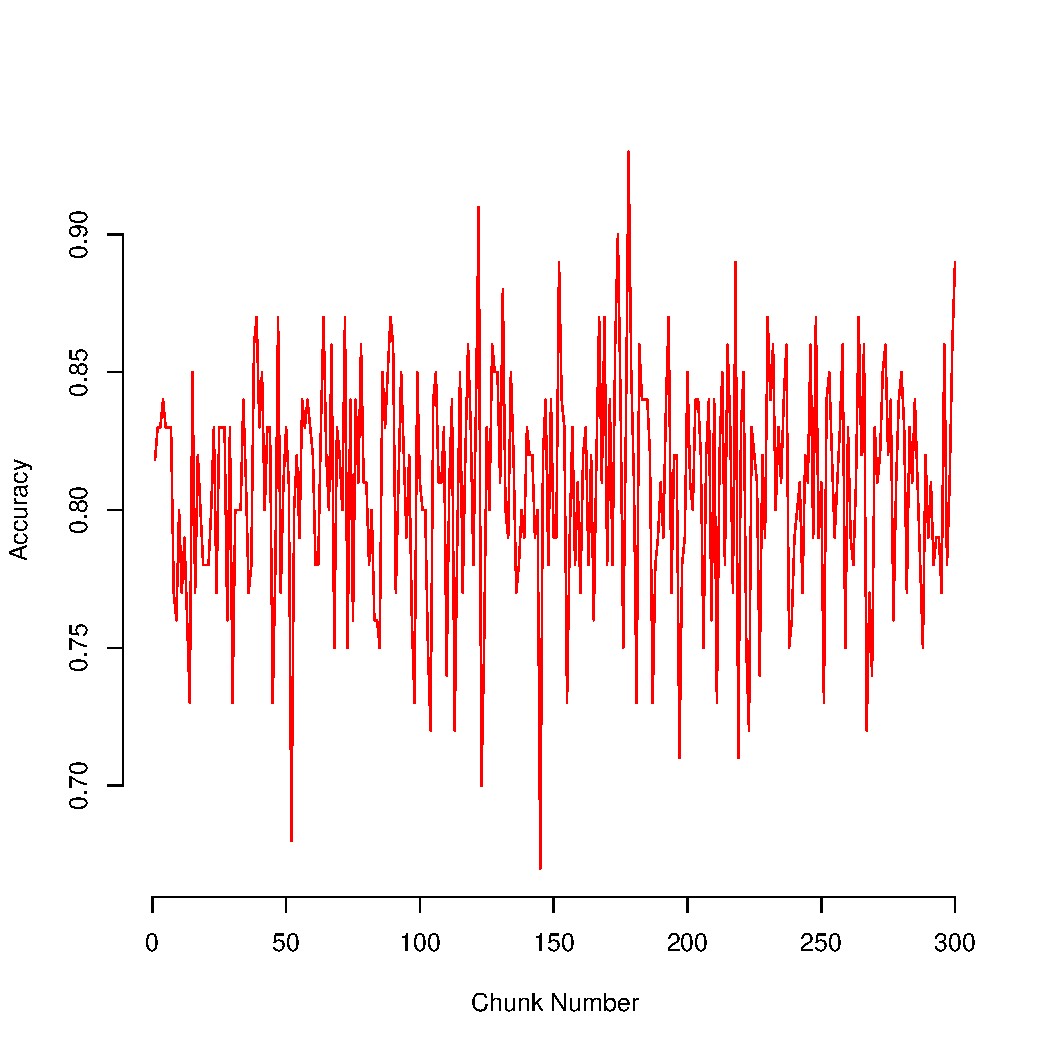
\includegraphics[width=\maxwidth]{figure/unnamed-chunk-65-1} 

\end{knitrout}
\caption {Chunk Number vs Accuracy}
\label{fig2}
\end {center}
\end {figure}

As the plot above shows, the overall accuracy varies as the chunk number increases. Although it drops to bellow 70\% just after 50 chunks and again just before 150 chunks. The highest accuracy value is between 170 and 190 chunks.

The limitation for data streaming is that the adult dataset is unbalanced, also to improve classification models more computing resources would be required. As this is a length process that is restricted to the computing power provided on my laptop.

\clearpage

\section {Text Classification}
For this task a csv of leave/remain tweets of the brexit campaign was provided.

The was first imported:
\begin{knitrout}
\definecolor{shadecolor}{rgb}{0.969, 0.969, 0.969}\color{fgcolor}\begin{kframe}
\begin{alltt}
\hlstd{leaveRemainTweets} \hlkwb{<-} \hlkwd{read.csv}\hlstd{(}\hlstr{"data/leaveRemainTweets_CW.csv"}\hlstd{,} \hlkwc{header}\hlstd{=}\hlnum{TRUE}\hlstd{)}
\end{alltt}
\end{kframe}
\end{knitrout}



Then the tweets are split based on the label(leave/remain)

\begin{knitrout}
\definecolor{shadecolor}{rgb}{0.969, 0.969, 0.969}\color{fgcolor}\begin{kframe}
\begin{alltt}
\hlcom{#split dataset into leave and remain dataframes}
\hlstd{tweets} \hlkwb{=} \hlkwd{split}\hlstd{(leaveRemainTweets, leaveRemainTweets}\hlopt{$}\hlstd{label)}
\hlstd{remainTweets} \hlkwb{=} \hlstd{tweets}\hlopt{$}\hlstd{Remain}
\hlstd{leaveTweets} \hlkwb{=} \hlstd{tweets}\hlopt{$}\hlstd{Leave}
\end{alltt}
\end{kframe}
\end{knitrout}



Next lets check how many leave/remain tweets they are
\begin{knitrout}
\definecolor{shadecolor}{rgb}{0.969, 0.969, 0.969}\color{fgcolor}\begin{kframe}
\begin{alltt}
\hlkwd{nrow}\hlstd{(remainTweets)}
\hlkwd{nrow}\hlstd{(leaveTweets)}
\end{alltt}
\end{kframe}
\end{knitrout}

Number of remain tweets
\begin{knitrout}
\definecolor{shadecolor}{rgb}{0.969, 0.969, 0.969}\color{fgcolor}\begin{kframe}
\begin{verbatim}
## [1] 1029
\end{verbatim}
\end{kframe}
\end{knitrout}

Number of leave tweets
\begin{knitrout}
\definecolor{shadecolor}{rgb}{0.969, 0.969, 0.969}\color{fgcolor}\begin{kframe}
\begin{verbatim}
## [1] 1254
\end{verbatim}
\end{kframe}
\end{knitrout}


\subsection{Preprocessing}

In order to pre-process the leaveRemain tweets, I built a custom corpus function. Which can be found below.
\begin{knitrout}
\definecolor{shadecolor}{rgb}{0.969, 0.969, 0.969}\color{fgcolor}\begin{kframe}
\begin{alltt}
\hlstd{buildCorpus} \hlkwb{<-} \hlkwa{function} \hlstd{(}\hlkwc{tweets}\hlstd{,} \hlkwc{wordCloud}\hlstd{,} \hlkwc{wholeDataSet}\hlstd{,} \hlkwc{wordAssocation}\hlstd{,} \hlkwc{dtm}\hlstd{)\{}

  \hlcom{#Check the optional parameters are set}
  \hlstd{wordA} \hlkwb{<-}\hlkwd{hasArg}\hlstd{(wordAssocation)}
  \hlstd{wds} \hlkwb{<-} \hlkwd{hasArg}\hlstd{(wholeDataSet)}
  \hlstd{wordc} \hlkwb{<-}  \hlkwd{hasArg}\hlstd{(wordCloud)}
  \hlstd{dtmcheck} \hlkwb{<-} \hlkwd{hasArg}\hlstd{(dtm)}

  \hlstd{corp} \hlkwb{<-} \hlkwd{Corpus}\hlstd{(}\hlkwd{VectorSource}\hlstd{(tweets}\hlopt{$}\hlstd{text))}


  \hlstd{corp} \hlkwb{<-} \hlkwd{tm_map}\hlstd{(corp,}
                 \hlkwd{content_transformer}\hlstd{(}\hlkwa{function}\hlstd{(}\hlkwc{x}\hlstd{)} \hlkwd{iconv}\hlstd{(x,} \hlkwc{to}\hlstd{=}\hlstr{'ASCII'}\hlstd{,}
                                                       \hlkwc{sub}\hlstd{=}\hlstr{'byte'}\hlstd{)))}
  \hlcom{# remove stop words and other preprocessing}

  \hlstd{corp} \hlkwb{<-} \hlkwd{tm_map}\hlstd{(corp,} \hlkwd{content_transformer}\hlstd{(tolower))}
  \hlstd{corp} \hlkwb{<-} \hlkwd{tm_map}\hlstd{(corp, removeNumbers)}

  \hlstd{toSpace} \hlkwb{=} \hlkwd{content_transformer}\hlstd{(} \hlkwa{function}\hlstd{(}\hlkwc{x}\hlstd{,} \hlkwc{pattern}\hlstd{)} \hlkwd{gsub}\hlstd{(pattern,}\hlstr{" "}\hlstd{,x) )}


  \hlcom{##Tweet cleaning}

  \hlcom{#credit to https://stackoverflow.com/a/31352005/8816204}
  \hlstd{corp} \hlkwb{<-}\hlkwd{tm_map}\hlstd{(corp, toSpace,} \hlstr{"(RT|via)((?:\textbackslash{}\textbackslash{}b\textbackslash{}\textbackslash{}W*@\textbackslash{}\textbackslash{}w+)+)"}\hlstd{)}
  \hlstd{corp} \hlkwb{<-}\hlkwd{tm_map}\hlstd{(corp, toSpace,} \hlstr{"@\textbackslash{}\textbackslash{}w+"}\hlstd{)}
  \hlstd{corp} \hlkwb{<-}\hlkwd{tm_map}\hlstd{(corp, toSpace,} \hlstr{"&amp"}\hlstd{)}

  \hlcom{##Remove URLS from tweets}
  \hlstd{corp} \hlkwb{<-}\hlkwd{tm_map}\hlstd{(corp, toSpace,} \hlstr{"httpsw+"}\hlstd{)}
  \hlstd{corp} \hlkwb{<-}\hlkwd{tm_map}\hlstd{(corp, toSpace,} \hlstr{"http:\textbackslash{}\textbackslash{}w+"}\hlstd{)}
  \hlstd{corp} \hlkwb{<-}\hlkwd{tm_map}\hlstd{(corp, toSpace,} \hlstr{"https:\textbackslash{}\textbackslash{}w+"}\hlstd{)}

  \hlstd{corp} \hlkwb{<-}\hlkwd{tm_map}\hlstd{(corp, toSpace,} \hlstr{"[ \textbackslash{}t]\{2,\}"}\hlstd{)}
  \hlstd{corp} \hlkwb{<-}\hlkwd{tm_map}\hlstd{(corp, toSpace,} \hlstr{"^\textbackslash{}\textbackslash{}s+|\textbackslash{}\textbackslash{}s+$"}\hlstd{)}


  \hlcom{# ##Remove obvious words /stopwords}
  \hlkwa{if}\hlstd{(wds)\{}
    \hlkwa{if}\hlstd{(wholeDataSet)\{}
      \hlstd{corp} \hlkwb{<-} \hlkwd{tm_map}\hlstd{(corp,} \hlkwa{function}\hlstd{(}\hlkwc{x}\hlstd{)}\hlkwd{removeWords}
                     \hlstd{(x,}\hlkwd{c}\hlstd{(}\hlkwd{stopwords}\hlstd{(}\hlstr{"english"}\hlstd{),}\hlstr{"amp"}\hlstd{,} \hlstr{"will"}\hlstd{,} \hlstr{"‰Û_"}\hlstd{,} \hlstr{"https"}\hlstd{,} \hlstr{"http"}\hlstd{,} \hlstr{"httpsdb"}
                          \hlstd{,} \hlstr{"eu"}\hlstd{,} \hlstr{"brexit"}\hlstd{,} \hlstr{"rt"}\hlstd{,} \hlstr{"leave"}\hlstd{,} \hlstr{"remain"}\hlstd{,} \hlstr{"vote"}\hlstd{)))}
    \hlstd{\}}
  \hlstd{\}}
  \hlkwa{else}\hlstd{\{}
    \hlstd{corp} \hlkwb{<-} \hlkwd{tm_map}\hlstd{(corp,} \hlkwa{function}\hlstd{(}\hlkwc{x}\hlstd{)}\hlkwd{removeWords}
                   \hlstd{(x,}\hlkwd{c}\hlstd{(}\hlkwd{stopwords}\hlstd{(}\hlstr{"english"}\hlstd{),}\hlstr{"amp"}\hlstd{,} \hlstr{"will"}\hlstd{,} \hlstr{"‰Û_"}\hlstd{,} \hlstr{"https"}\hlstd{,} \hlstr{"http"}\hlstd{,} \hlstr{"httpsdb"}\hlstd{)))}
  \hlstd{\}}



  \hlcom{#remove punctuation last so urls are removed correctly}
  \hlstd{corp} \hlkwb{<-} \hlkwd{tm_map}\hlstd{(corp, removePunctuation)}


  \hlcom{#If wordAssocation is true then create term document  matrix}
  \hlkwa{if}\hlstd{(wordA)\{}
    \hlkwa{if}\hlstd{(wordAssocation)\{}
      \hlstd{tdm} \hlkwb{<-} \hlkwd{TermDocumentMatrix}\hlstd{(corp)}
    \hlstd{\}}
    \hlkwa{else}\hlstd{\{}
      \hlkwa{if}\hlstd{(dtm)\{}  \hlcom{# if dtm is true the create document term matrix}
        \hlstd{dtm} \hlkwb{<-} \hlkwd{DocumentTermMatrix}\hlstd{(corp)}
      \hlstd{\}}
    \hlstd{\}}

  \hlstd{\}}

  \hlkwa{else if}\hlstd{(}\hlopt{!}\hlstd{wordA)\{} \hlcom{# If no  wordAssocation then create TermDocument Matrix}
    \hlstd{tdm} \hlkwb{<-} \hlkwd{TermDocumentMatrix}\hlstd{(corp)}

    \hlstd{m} \hlkwb{<-} \hlkwd{as.matrix}\hlstd{(tdm)}
    \hlstd{v} \hlkwb{<-} \hlkwd{sort}\hlstd{(}\hlkwd{rowSums}\hlstd{(m),} \hlkwc{decreasing} \hlstd{=} \hlnum{TRUE}\hlstd{)}
    \hlstd{d} \hlkwb{<-} \hlkwd{data.frame}\hlstd{(}\hlkwc{word} \hlstd{=} \hlkwd{names}\hlstd{(v),} \hlkwc{freq} \hlstd{= v)}
    \hlstd{d}\hlopt{$}\hlstd{word} \hlkwb{<-} \hlkwd{gsub}\hlstd{(}\hlstr{"˜"}\hlstd{,} \hlstr{" "}\hlstd{, d}\hlopt{$}\hlstd{word)} \hlcom{## Edit 2}


    \hlkwa{if}\hlstd{(wordc)\{}
      \hlkwa{if}\hlstd{(wds)\{}
        \hlstd{tweets} \hlkwb{<-} \hlstd{d}\hlopt{$}\hlstd{word} \hlcom{#whole dataset return df of processed tweets}
      \hlstd{\}} \hlkwa{else}\hlstd{\{}
        \hlstd{tweets} \hlkwb{<-} \hlstd{d}\hlopt{$}\hlstd{word}
        \hlkwa{if}\hlstd{(wordCloud)\{} \hlcom{#return wordcloud if TRUE}
          \hlkwd{wordcloud}\hlstd{(}\hlkwc{words} \hlstd{=tweets,} \hlkwc{freq} \hlstd{= d}\hlopt{$}\hlstd{freq,} \hlkwc{min.freq} \hlstd{=} \hlnum{3}\hlstd{,}
                    \hlkwc{max.words}\hlstd{=}\hlnum{2000}\hlstd{,} \hlkwc{random.order}\hlstd{=}\hlnum{FALSE}\hlstd{,} \hlkwc{rot.per}\hlstd{=}\hlnum{0.2}\hlstd{,}
                    \hlkwc{colors}\hlstd{=}\hlkwd{brewer.pal}\hlstd{(}\hlnum{8}\hlstd{,} \hlstr{"Dark2"}\hlstd{))}
        \hlstd{\}}
      \hlstd{\}}

    \hlstd{\}}

  \hlstd{\}}

\hlstd{\}}
\end{alltt}
\end{kframe}
\end{knitrout}



By using the buildCorpus function with the word cloud parameter set to TRUE, it will create a word cloud for us. 
\begin{knitrout}
\definecolor{shadecolor}{rgb}{0.969, 0.969, 0.969}\color{fgcolor}\begin{kframe}
\begin{alltt}
\hlstd{leaveWordCloud} \hlkwb{<-} \hlkwd{buildCorpus}\hlstd{(leaveTweets,}\hlnum{TRUE}\hlstd{)}

\hlstd{remainWordCloud} \hlkwb{<-} \hlkwd{buildCorpus}\hlstd{(remainTweets,}\hlnum{TRUE}\hlstd{)}
\end{alltt}
\end{kframe}
\end{knitrout}

Please see (Figure~\ref{fig3}) for leave tweets word cloud and (Figure~\ref{fig4}) for remain tweets wordcloud.

\begin{figure}[H]
\begin{center}
\begin{knitrout}
\definecolor{shadecolor}{rgb}{0.969, 0.969, 0.969}\color{fgcolor}
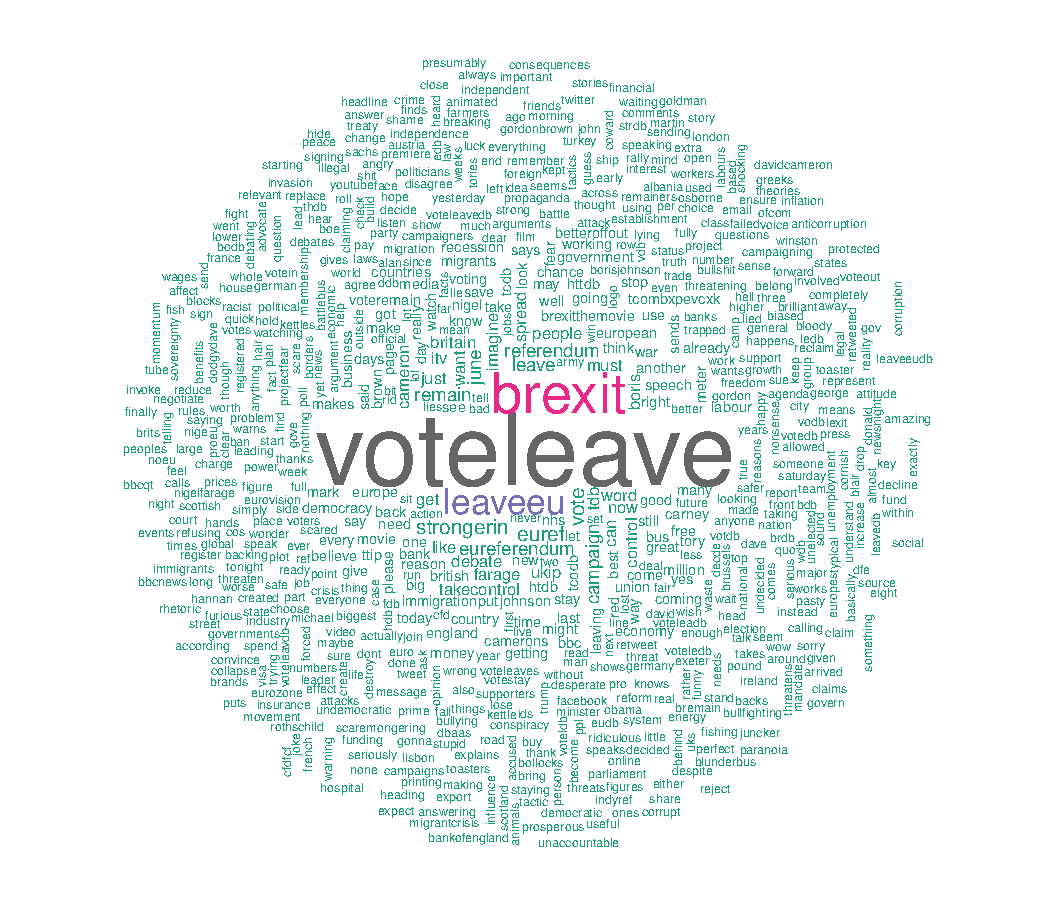
\includegraphics[width=.80\linewidth]{figure/unnamed-chunk-76-1} 

\end{knitrout}
\caption {Word cloud of leave tweets}
\label{fig3}
\end {center}
\end {figure}


\begin{figure}[H]
\begin{center}
\begin{knitrout}
\definecolor{shadecolor}{rgb}{0.969, 0.969, 0.969}\color{fgcolor}
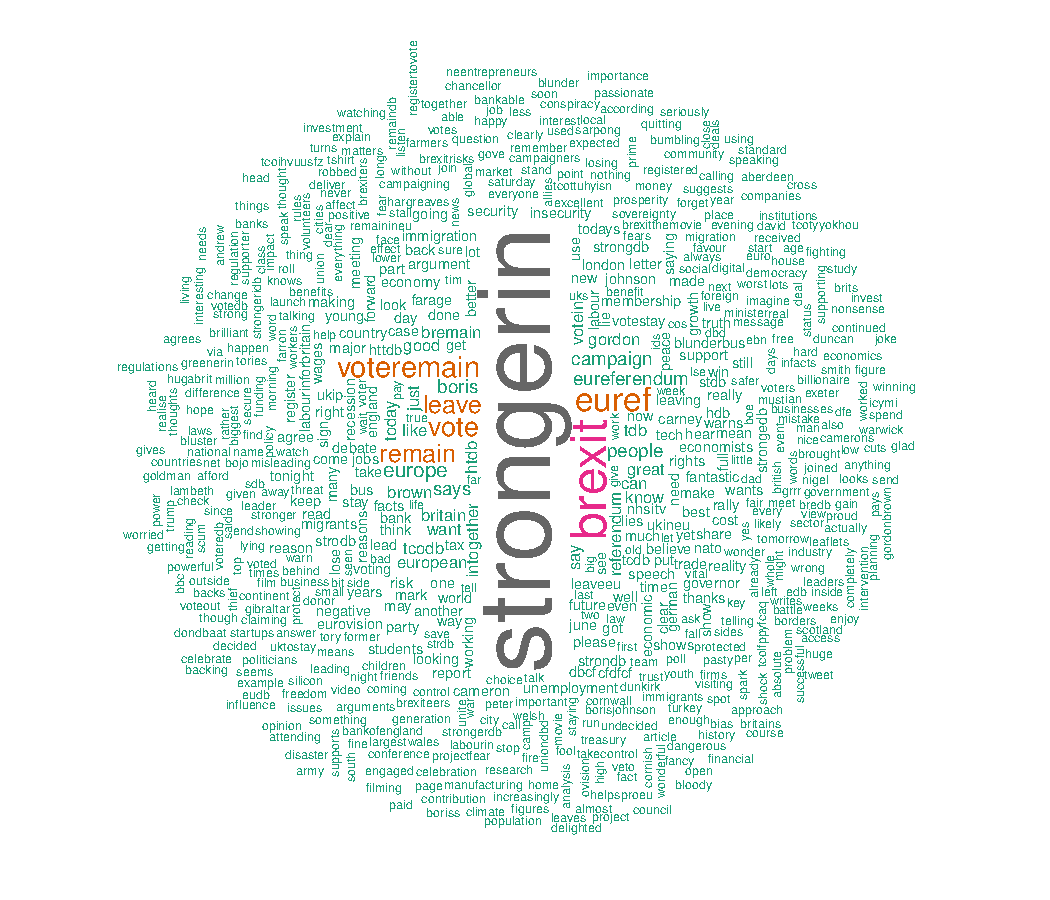
\includegraphics[width=.80\linewidth]{figure/unnamed-chunk-77-1} 

\end{knitrout}
\caption {Word cloud of Remain tweets}
\label{fig4}
\end {center}
\end {figure}


\clearpage


\subsection{Text Analysis}

\subsubsection{Most Frequent word in Tweet Collection}

To find the most frequent word in the collection of tweets, the whole leaveRemainTweets dataframe was based into the buildCorpus function with the wordCloud option set to FALSE and wholedataset option set to TRUE.

\begin{knitrout}
\definecolor{shadecolor}{rgb}{0.969, 0.969, 0.969}\color{fgcolor}\begin{kframe}
\begin{alltt}
\hlcom{#Get Most frequent word}
\hlstd{tweetWordCloud} \hlkwb{<-}\hlkwd{buildCorpus}\hlstd{(leaveRemainTweets,} \hlnum{FALSE}\hlstd{,} \hlnum{TRUE}\hlstd{)}
\hlkwd{head}\hlstd{(tweetWordCloud,}\hlnum{1}\hlstd{)}
\end{alltt}
\end{kframe}
\end{knitrout}


\begin{knitrout}
\definecolor{shadecolor}{rgb}{0.969, 0.969, 0.969}\color{fgcolor}\begin{kframe}
\begin{verbatim}
## [1] "voteleave"
\end{verbatim}
\end{kframe}
\end{knitrout}


\subsubsection{Word Association}


To find out which words appear together often, I used the buildCorpus function to return a termDocumentMatrix. The most frequent terms with a lowfreq value of 50 is also created.

\begin{knitrout}
\definecolor{shadecolor}{rgb}{0.969, 0.969, 0.969}\color{fgcolor}\begin{kframe}
\begin{alltt}
\hlstd{wordAssoication} \hlkwb{<-} \hlkwd{buildCorpus}\hlstd{(leaveRemainTweets,}\hlnum{FALSE}\hlstd{,}\hlnum{TRUE}\hlstd{,}\hlnum{TRUE}\hlstd{)}
\hlstd{freq.terms} \hlkwb{<-} \hlkwd{findFreqTerms}\hlstd{(wordAssoication,} \hlkwc{lowfreq} \hlstd{=}\hlnum{50}\hlstd{)}
\end{alltt}
\end{kframe}
\end{knitrout}





Lets inspect the top 30 most frequent words in the tweet collection


\begin{knitrout}
\definecolor{shadecolor}{rgb}{0.969, 0.969, 0.969}\color{fgcolor}\begin{kframe}
\begin{alltt}
\hlkwd{head}\hlstd{(freq.terms,}\hlnum{30}\hlstd{)}
\end{alltt}
\end{kframe}
\end{knitrout}

\begin{knitrout}
\definecolor{shadecolor}{rgb}{0.969, 0.969, 0.969}\color{fgcolor}\begin{kframe}
\begin{verbatim}
##  [1] "strongerin"   "voteleave"    "referendum"   "tdb"         
##  [5] "boris"        "says"         "leaveeu"      "like"        
##  [9] "tcodb"        "want"         "europe"       "get"         
## [13] "britain"      "know"         "imagine"      "june"        
## [17] "now"          "euref"        "eureferendum" "think"       
## [21] "can"          "campaign"     "voteremain"   "debate"      
## [25] "farage"       "just"         "must"         "people"      
## [29] "european"     "good"
\end{verbatim}
\end{kframe}
\end{knitrout}

Now to plot (Figure~\ref{fig5}) the word association (term document matrix) against the frequent terms.
\begin{knitrout}
\definecolor{shadecolor}{rgb}{0.969, 0.969, 0.969}\color{fgcolor}\begin{kframe}
\begin{alltt}
\hlkwd{plot}\hlstd{(wordAssoication,} \hlkwc{term} \hlstd{= freq.terms,} \hlkwc{corThreshold} \hlstd{=} \hlnum{0.12}\hlstd{,} \hlkwc{weighting} \hlstd{= T)}
\end{alltt}
\end{kframe}
\end{knitrout}

In the plot, the thicker the line between words the greater the association. In this case June as a strong association with imagine and vote leave.

Similar with European with 'must' and 'now'. Also 'Farage' and 'debate'.

\begin{figure}[H]
\begin{center}
\includegraphics[page=1,width=.90\textwidth]{{wordAPlot.pdf}}
\caption {Word Association Plot}
\label{fig5}
\end {center}
\end {figure}



% 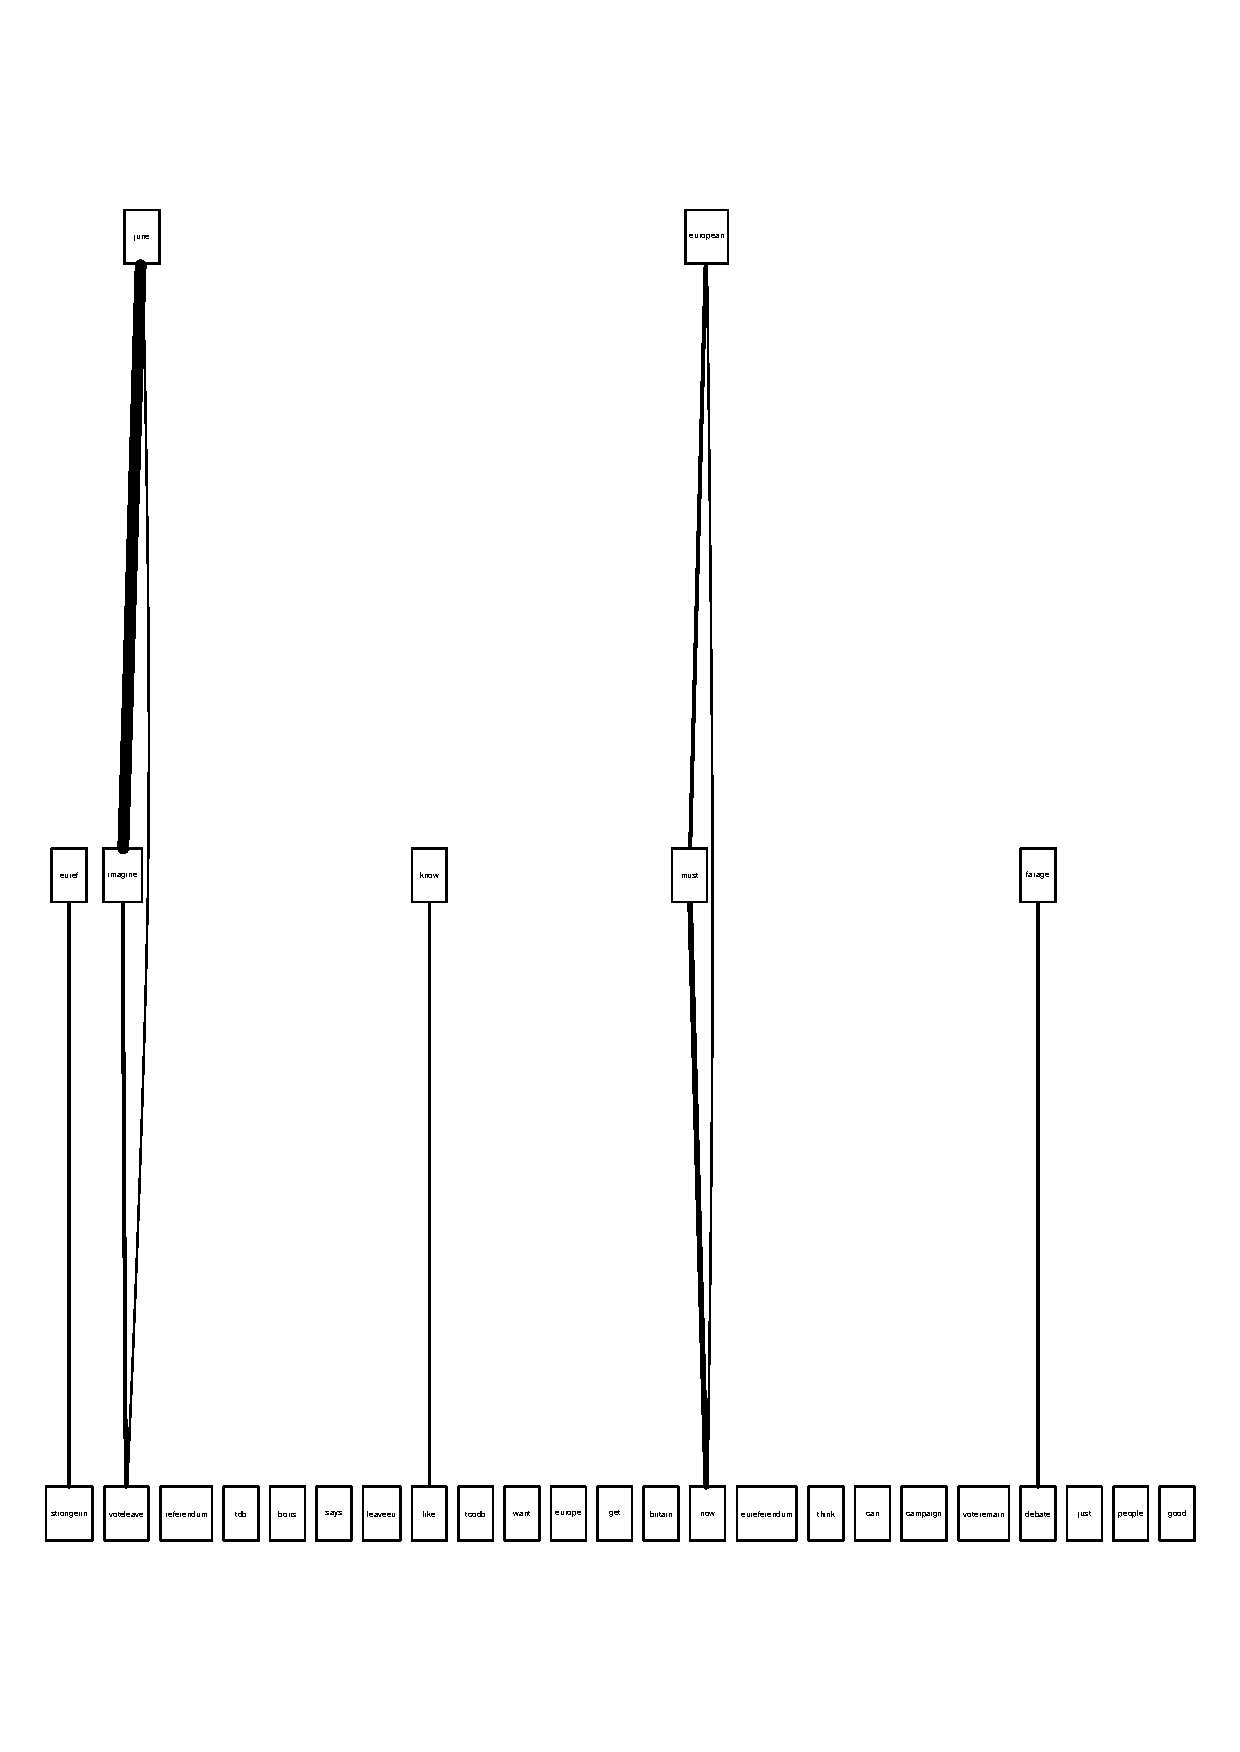
\includepdf[pages={1-},scale=0.75]{wordAPlot.pdf}




\subsubsection{Most Frequent Words in Both Leave \& Remain Tweets}

\begin{knitrout}
\definecolor{shadecolor}{rgb}{0.969, 0.969, 0.969}\color{fgcolor}\begin{kframe}
\begin{alltt}
\hlcom{#Leave}
\hlstd{leaveWords} \hlkwb{<-} \hlkwd{buildCorpus}\hlstd{(leaveTweets,} \hlnum{FALSE}\hlstd{,}\hlnum{TRUE}\hlstd{)}
\hlkwd{head}\hlstd{(leaveWords,} \hlnum{10}\hlstd{)}
\end{alltt}
\end{kframe}
\end{knitrout}

\begin{knitrout}
\definecolor{shadecolor}{rgb}{0.969, 0.969, 0.969}\color{fgcolor}\begin{kframe}
\begin{verbatim}
##  [1] "voteleave"    "leaveeu"      "strongerin"   "euref"       
##  [5] "eureferendum" "june"         "referendum"   "campaign"    
##  [9] "now"          "people"
\end{verbatim}
\end{kframe}
\end{knitrout}


\begin{knitrout}
\definecolor{shadecolor}{rgb}{0.969, 0.969, 0.969}\color{fgcolor}\begin{kframe}
\begin{alltt}
\hlcom{#Remain}
\hlstd{remainWords} \hlkwb{<-} \hlkwd{buildCorpus}\hlstd{(remainTweets,} \hlnum{FALSE}\hlstd{,}\hlnum{TRUE}\hlstd{)}
\hlkwd{head}\hlstd{(remainWords,} \hlnum{10}\hlstd{)}
\end{alltt}
\end{kframe}
\end{knitrout}

\begin{knitrout}
\definecolor{shadecolor}{rgb}{0.969, 0.969, 0.969}\color{fgcolor}\begin{kframe}
\begin{verbatim}
##  [1] "strongerin"   "euref"        "voteremain"   "europe"      
##  [5] "says"         "eureferendum" "campaign"     "people"      
##  [9] "boris"        "britain"
\end{verbatim}
\end{kframe}
\end{knitrout}

\clearpage

\subsection{Text Classification}

\subsubsection{kNNModel}

\begin{knitrout}
\definecolor{shadecolor}{rgb}{0.969, 0.969, 0.969}\color{fgcolor}\begin{kframe}
\begin{alltt}
\hlstd{dtm} \hlkwb{<-}  \hlkwd{buildCorpus}\hlstd{(leaveRemainTweets,}\hlnum{FALSE}\hlstd{,}\hlnum{TRUE}\hlstd{,}\hlnum{FALSE}\hlstd{,}\hlnum{TRUE}\hlstd{)}

\hlstd{dtm} \hlkwb{<-} \hlkwd{as.matrix}\hlstd{(dtm)}
\hlstd{tweets} \hlkwb{<-} \hlkwd{data.frame}\hlstd{(dtm)}

\hlstd{tweets}\hlopt{$}\hlstd{label} \hlkwb{<-} \hlstd{leaveRemainTweets}\hlopt{$}\hlstd{label}
\end{alltt}
\end{kframe}
\end{knitrout}




\begin{knitrout}
\definecolor{shadecolor}{rgb}{0.969, 0.969, 0.969}\color{fgcolor}\begin{kframe}
\begin{alltt}
\hlcom{#Split data into training and testing subsets}
\hlcom{#Divide the dataset into 70% training and 30% testing, to prevent overfitting from occurring}
\hlstd{inTrainTweets} \hlkwb{<-} \hlkwd{createDataPartition}\hlstd{(}\hlkwc{y}\hlstd{=tweets}\hlopt{$}\hlstd{label,} \hlkwc{p}\hlstd{=}\hlnum{0.7}\hlstd{,} \hlkwc{list}\hlstd{=}\hlnum{FALSE}\hlstd{)}

\hlcom{#Assign indexes to split the Tweets DTM into training and testing}
\hlstd{training} \hlkwb{<-} \hlstd{tweets[inTrainTweets,]}
\hlstd{testing} \hlkwb{<-} \hlstd{tweets[}\hlopt{-}\hlstd{inTrainTweets,]}
\end{alltt}
\end{kframe}
\end{knitrout}




\begin{knitrout}
\definecolor{shadecolor}{rgb}{0.969, 0.969, 0.969}\color{fgcolor}\begin{kframe}
\begin{alltt}
\hlstd{train_control}\hlkwb{<-} \hlkwd{trainControl}\hlstd{(}\hlkwc{method}\hlstd{=}\hlstr{"cv"}\hlstd{,} \hlkwc{number}\hlstd{=}\hlnum{5}\hlstd{,}\hlkwc{verboseIter}\hlstd{=}\hlnum{FALSE}\hlstd{)}

\hlstd{kNNTweets} \hlkwb{<-} \hlkwd{train}\hlstd{(label}\hlopt{~}\hlstd{.,} \hlkwc{data} \hlstd{= training,}
                  \hlkwc{trControl} \hlstd{= train_control,}
                  \hlkwc{tuneLength} \hlstd{=}\hlnum{5}\hlstd{,}
                  \hlkwc{method} \hlstd{=} \hlstr{"knn"}

\hlstd{)}
\end{alltt}
\end{kframe}
\end{knitrout}





\begin{knitrout}
\definecolor{shadecolor}{rgb}{0.969, 0.969, 0.969}\color{fgcolor}\begin{kframe}
\begin{alltt}
\hlstd{kNNTweets}
\end{alltt}
\end{kframe}
\end{knitrout}

\begin{knitrout}
\definecolor{shadecolor}{rgb}{0.969, 0.969, 0.969}\color{fgcolor}\begin{kframe}
\begin{verbatim}
## k-Nearest Neighbors 
## 
## 1599 samples
## 6027 predictors
##    2 classes: 'Leave', 'Remain' 
## 
## No pre-processing
## Resampling: Cross-Validated (5 fold) 
## Summary of sample sizes: 1280, 1280, 1278, 1279, 1279 
## Resampling results across tuning parameters:
## 
##   k   Accuracy   Kappa    
##    5  0.8480166  0.6848774
##    7  0.8423955  0.6728668
##    9  0.8442646  0.6769512
##   11  0.8455068  0.6795951
##   13  0.8417646  0.6717658
## 
## Accuracy was used to select the optimal model using the largest value.
## The final value used for the model was k = 5.
\end{verbatim}
\end{kframe}
\end{knitrout}

\begin{knitrout}
\definecolor{shadecolor}{rgb}{0.969, 0.969, 0.969}\color{fgcolor}\begin{kframe}
\begin{alltt}
\hlcom{#Evaluate}

\hlstd{predictkNNTweets} \hlkwb{<-} \hlkwd{predict}\hlstd{(kNNTweets,testing)}
\hlkwd{confusionMatrix}\hlstd{(predictkNNTweets, testing}\hlopt{$}\hlstd{label)}
\end{alltt}
\end{kframe}
\end{knitrout}

\begin{knitrout}
\definecolor{shadecolor}{rgb}{0.969, 0.969, 0.969}\color{fgcolor}\begin{kframe}
\begin{verbatim}
## Confusion Matrix and Statistics
## 
##           Reference
## Prediction Leave Remain
##     Leave    372    108
##     Remain     4    200
##                                           
##                Accuracy : 0.8363          
##                  95% CI : (0.8064, 0.8632)
##     No Information Rate : 0.5497          
##     P-Value [Acc > NIR] : < 2.2e-16       
##                                           
##                   Kappa : 0.6588          
##  Mcnemar's Test P-Value : < 2.2e-16       
##                                           
##             Sensitivity : 0.9894          
##             Specificity : 0.6494          
##          Pos Pred Value : 0.7750          
##          Neg Pred Value : 0.9804          
##              Prevalence : 0.5497          
##          Detection Rate : 0.5439          
##    Detection Prevalence : 0.7018          
##       Balanced Accuracy : 0.8194          
##                                           
##        'Positive' Class : Leave           
## 
\end{verbatim}
\end{kframe}
\end{knitrout}


\clearpage

\subsubsection{Improved SVM Model}

\begin{knitrout}
\definecolor{shadecolor}{rgb}{0.969, 0.969, 0.969}\color{fgcolor}\begin{kframe}
\begin{alltt}
\hlcom{#Set Train Control to cross-validation 5 fold}
\hlstd{train_control}\hlkwb{<-} \hlkwd{trainControl}\hlstd{(}\hlkwc{method}\hlstd{=}\hlstr{"cv"}\hlstd{,} \hlkwc{number}\hlstd{=}\hlnum{5}\hlstd{,}\hlkwc{verboseIter}\hlstd{=}\hlnum{FALSE}\hlstd{)}

\hlcom{#Set model to SVM with tunelength of 10}

\hlstd{svmModel} \hlkwb{<-} \hlkwd{train}\hlstd{(label}\hlopt{~} \hlstd{.,} \hlkwc{data} \hlstd{= training,}
                  \hlkwc{trControl} \hlstd{= train_control,}
                  \hlkwc{tuneLength} \hlstd{=}\hlnum{10}\hlstd{,}
                  \hlkwc{method} \hlstd{=} \hlstr{"svmRadial"}

\hlstd{)}
\end{alltt}
\end{kframe}
\end{knitrout}



\begin{knitrout}
\definecolor{shadecolor}{rgb}{0.969, 0.969, 0.969}\color{fgcolor}\begin{kframe}
\begin{alltt}
\hlstd{svmModel}
\end{alltt}
\end{kframe}
\end{knitrout}

\begin{knitrout}
\definecolor{shadecolor}{rgb}{0.969, 0.969, 0.969}\color{fgcolor}\begin{kframe}
\begin{verbatim}
## Support Vector Machines with Radial Basis Function Kernel 
## 
## 1599 samples
## 6027 predictors
##    2 classes: 'Leave', 'Remain' 
## 
## No pre-processing
## Resampling: Cross-Validated (5 fold) 
## Summary of sample sizes: 1279, 1279, 1278, 1280, 1280 
## Resampling results across tuning parameters:
## 
##   C       Accuracy   Kappa    
##     0.25  0.8986713  0.7986826
##     0.50  0.8949076  0.7912300
##     1.00  0.8967806  0.7946679
##     2.00  0.9024134  0.8043444
##     4.00  0.9049076  0.8093912
##     8.00  0.9049076  0.8093912
##    16.00  0.9049076  0.8093912
##    32.00  0.9049076  0.8093912
##    64.00  0.9049076  0.8093912
##   128.00  0.9049076  0.8093912
## 
## Tuning parameter 'sigma' was held constant at a value of 0.06818182
## Accuracy was used to select the optimal model using the largest value.
## The final values used for the model were sigma = 0.06818182 and C = 4.
\end{verbatim}
\end{kframe}
\end{knitrout}

\begin{knitrout}
\definecolor{shadecolor}{rgb}{0.969, 0.969, 0.969}\color{fgcolor}\begin{kframe}
\begin{alltt}
\hlcom{#Evaluate}

\hlstd{predictSVM} \hlkwb{<-} \hlkwd{predict}\hlstd{(svmModel,testing)}
\hlkwd{confusionMatrix}\hlstd{(predictSVM, testing}\hlopt{$}\hlstd{label)}
\end{alltt}
\end{kframe}
\end{knitrout}

\begin{knitrout}
\definecolor{shadecolor}{rgb}{0.969, 0.969, 0.969}\color{fgcolor}\begin{kframe}
\begin{verbatim}
## Confusion Matrix and Statistics
## 
##           Reference
## Prediction Leave Remain
##     Leave    346     20
##     Remain    30    288
##                                           
##                Accuracy : 0.9269          
##                  95% CI : (0.9048, 0.9453)
##     No Information Rate : 0.5497          
##     P-Value [Acc > NIR] : <2e-16          
##                                           
##                   Kappa : 0.8528          
##  Mcnemar's Test P-Value : 0.2031          
##                                           
##             Sensitivity : 0.9202          
##             Specificity : 0.9351          
##          Pos Pred Value : 0.9454          
##          Neg Pred Value : 0.9057          
##              Prevalence : 0.5497          
##          Detection Rate : 0.5058          
##    Detection Prevalence : 0.5351          
##       Balanced Accuracy : 0.9276          
##                                           
##        'Positive' Class : Leave           
## 
\end{verbatim}
\end{kframe}
\end{knitrout}


\clearpage



% Clear the page and starte a new page for references 

\clearpage
% The title for the reference section is called References 

\section{References}\label{pubs}

\printbibliography[heading =none]


\clearpage


\end{document}
